%%%%%%%%%%%%%%%%%%%%%%%%%%%%%%%%%%%%%%%%%
% Journal Article
% LaTeX Template
% Version 2.0 (February 7, 2023)
%
% This template originates from:
% https://www.LaTeXTemplates.com
%
% Author:
% Vel (vel@latextemplates.com)
%
% License:
% CC BY-NC-SA 4.0 (https://creativecommons.org/licenses/by-nc-sa/4.0/)
%
% NOTE: The bibliography needs to be compiled using the biber engine.
%
%%%%%%%%%%%%%%%%%%%%%%%%%%%%%%%%%%%%%%%%%

%----------------------------------------------------------------------------------------
%	PACKAGES AND OTHER DOCUMENT CONFIGURATIONS
%----------------------------------------------------------------------------------------

\documentclass[
	a4paper, % Paper size, use either a4paper or letterpaper
	10pt, % Default font size, can also use 11pt or 12pt, although this is not recommended
	unnumberedsections, % Comment to enable section numbering
	twoside, % Two side traditional mode where headers and footers change between odd and even pages, comment this option to make them fixed
]{LTJournalArticle}

\addbibresource{bibliography.bib} % BibLaTeX bibliography file

\runninghead{Mitigating the effects of air bubbles on glider data to investigate productivity around Southern Ocean seamounts} % A shortened article title to appear in the running head, leave this command empty for no running head

\footertext{} % Text to appear in the footer, leave this command empty for no footer text

\usepackage{subcaption}

%----------------------------------------------------------------------------------------

\begin{document}

% \begin{figure}[h]
% 	\centering
% 	\includegraphics[width=0.2\textwidth]{Louis/figures/ucam-logo-colour-preferred.png} % Adjust the path to the image file
% 	\label{fig:ucam_logo}
% \end{figure}

% \maketitle % Output the title section
\begin{titlepage}
    \begin{center}
        \vspace*{2cm}
		
        \Huge
        \textbf{Mitigating the effects of air bubbles on glider data to investigate productivity around Southern Ocean seamounts}

        
		\vspace{3cm}

		\noindent
		\includegraphics[width=0.2\textwidth]{Louis/figures/University_Crest.pdf}
		\vspace{2cm}
		\Huge
        \\Louis De Neve\\
		\vspace{0.7cm}
		\Large
		Department of Applied Maths and Theoretical Physics\\
		University of Cambridge\\
		\vfill
        This thesis is submitted for the degree of\\
		\huge
        \textit{Master in Science\\}
		
        
		% \includegraphics[width=0.4\textwidth]{Louis/figures/ucam-logo-colour-preferred.png}
		% \vspace{0.8cm}
        % \Large
        % \\Department of Applied Maths and Theoretical Physics\\
        % University of Cambridge, UK\\
		% \vspace{0.8cm}
		% \includegraphics[width=0.4\textwidth]{Louis/figures/bas_colour_(transparent-png).png}
		% \vspace{0.8cm}
		% \\British Antarctic Survey, Cambridge, UK\\
		\huge
		\vspace{2cm}
        Easter 2025

		\large
		\vspace{0.5cm}
		Word count: 7098

		
		
    \end{center}
\end{titlepage}

\setcounter{page}{1}
\thispagestyle{plain}

	\begin{center} \Large Mitigating the effects of air bubbles on glider data to investigate productivity around Southern Ocean seamounts
	\end{center}

	\begin{abstract}
		\noindent Phytoplankton-driven biological productivity influences carbon sequestration from the surface into the deep ocean.
		By using buoyancy glider data from Discovery Bank in the South Scotia Ridge, this thesis investigates the impact of Taylor
		columns, hydrodynamic structures that form around seamounts, on this productivity. Air bubbles in water present a challenge
		to glider based bio-optical measurements by artificially inflating particulate backscattering coefficient readings,
		on the downward portion of the glider path. This thesis presents a novel method for mitigating the impact of
		bubbles on this data by applying a correction based on nearby unaffected upcasts, reducing the difference between up and
		downcasts by a factor of 6. The corrected data then reveals regions where high chlorophyll concentrations extend beyond the
		photic depth. These regions occur along the boundaries of the proposed Taylor column location, indicating increased nutrient
		upwelling and enhanced diapycnal mixing. The centre of the column does not show this effect, suggesting that increased water
		residence time in the centre of the column competes with the enhanced diapycnal mixing to limit nutrient availability and
		productivity. The findings suggest that the Taylor column significantly affects the productivity around Discovery Bank,
		highlighting the importance of accurate carbon sinking flux calculations to inform global climate policy decisions. 
		\vspace{0.2cm}
	\end{abstract}

%----------------------------------------------------------------------------------------
%	ARTICLE CONTENTS
%----------------------------------------------------------------------------------------

\begin{multicols}{2}

\section{1. Introduction}

With the ocean containing 60 times as much carbon as the atmosphere \citep{ref44}, a thorough understanding of oceanic systems
is needed to help guide climate policy decisions. The flux of carbon down into the deep ocean affects how much carbon is stored
within the ocean, with the most significant factor affecting this being the primary productivity of phytoplankton, by which CO$_2$,
or its derivatives, is converted into Particulate Organic Carbon (POC) \citep{ref45}. This primary biological productivity
(hereafter referred to as “productivity”) is in turn affected by a multitude of factors including temperature, the biota present
in a region and the availability of key nutrients - within the Southern Ocean the primary limiting nutrient is iron \citep{ref51}.
Hydrodynamic structures can have an effect on productivity by changing the availability of these key nutrients.
Taylor columns are a fluid dynamic phenomenon where the perturbation of a rotating fluid by a solid body creates rotating
columns parallel to the rotation axis \citep{ref47}. In the ocean, these columns can form around seamounts, large underwater
mountains that do not breach the surface. Taylor columns have been shown to affect the mixing of the ocean around seamounts
\citep{ref30}. Increased vertical mixing within the column results in more nutrients from below the euphotic zone being
brought up towards the surface, increasing productivity \citep{ref52}. This thesis aims to clarify the effect that undersea
topography has on this productivity by investigating the change in chlorophyll-$\alpha$ (henceforth referred to as “chlorophyll”)
concentrations and sinking particulate matter across transects over Discovery Bank, one of the largest seamounts in the South
Scotia Ridge.

The vast size of the ocean makes studying these systems incredibly difficult. Within the Southern Ocean this problem is compounded
by harsh weather and sea conditions, further exaggerated during the austral winter. In the past decade, buoyancy gliders have been
utilised to acquire ocean data across broad temporal and spatial ranges throughout the Southern Ocean. Buoyancy gliders have
recently become key tools for oceanographers to investigate biological and hydrodynamic systems within seas and oceans. Similar
to the Argo float programme \citep{ref59}, gliders do not need constant management, allowing them to conduct pre-programmed
routes and only requiring hands-on input from scientists during their deployment and recovery. This enables them to operate
independently from costly research vessels and cover larger regions than ever before. At the same time, gliders offer access
to regions previously inaccessible to ship-based measurements - they can approach within 50 meters of icebergs to take measurements
of water around these icebergs without the disturbance associated with large vessels \citep{ref48}. Gliders can be fitted with a
wide range of sensors, such as 3D scanning and sonar mapping sensors \citep{ref48, ref53}; conductivity, temperature and
depth sensors; acoustic fish and mammal detection; and optical sensors used to record fluorescence and other biological
properties of the water \citep{ref54, ref2}. The combination of high-precision data combined with control of the position of
the glider, a feature lacking on platforms such as the Argo floats, makes gliders suitable for a wide range of oceanographic
studies. 

Unfortunately, gliders are not without flaws: slow speeds and poor manoeuvrability make them vulnerable to strong currents
\citep{ref49}, while space and energy constraints can limit the options for science payloads. Bubbles also present a
problem for gliders utilising optical sensors, particularly sensors calculating volume backscattering functions to
calculate the turbidity of the water. For these sensors, bubbles refract the light in a similar way to particles but
the relation between volume scattering function and concentration is different, preventing accurate conversion. It is
important to confirm that the volume scattering functions do not contain signals from bubbles to ensure the conversion
to particle concentrations is reliable. In order to ascertain whether productivity around Discovery Bank is affected by
Taylor columns, we first need to investigate whether the effects of bubbles on backscattering data can be mitigated.
This thesis will suggest a method for reducing the erroneous high readings received from bubbles based on the difference
from other nearby unaffected readings.


\section{2. Literature Review}
\subsection{2.1. History of Gliders}
Gliders were first proposed as an alternative to propeller-driven underwater vehicles in the early 1960s by Concept Whisper,
an American military project constructed by General Dynamics aiming to provide a method of transporting military troops silently
through the ocean \citep{ref12}. The concept of buoyancy gliders was patented by Ewan Fallon \citep{ref13}, proposing the
sawtooth profile used by modern gliders, driven by a buoyancy engine. The potential uses of buoyancy gliders remained purely
military until the late 1980s when oceanographer Henry Stommel proposed a fleet of gliders to conduct oceanographic research,
nicknamed “The Slocum Mission” \citep{ref14}. The project was named after Joshua Slocum, the first person to single-handedly sail
around the world, indicating the global vision that Henry Stommel had for this project. In 1992 the University of Tokyo introduced
ALBAC, a drop weight glider that was only capable of a single glider cycle \citep{ref16}. In the late 1990s the US Office of Naval
Research produced three different gliders: Seaglider, Spray and Slocum \citep{ref15}. Produced by the Webb Research Corp (WRC) in
collaboration with Henry Stommel \citep{ref18}, the Slocum glider was initially created for shallow water missions as it was
powered by a single stroke pump, whose capacity limited the glider's operation in deeper water. By 2008, a later edition of the
glider, Slocum Thermal, solved these problems by using a Carnot cycle energy recovery system that utilizes the temperature gradient
between deep and surface waters to extract energy \citep{ref12}. Modern versions of the Slocum Thermal such as the Slocum Sentinel
now have endurances of up to 2 years \citep{ref27}, but are reliant on strong temperature gradients. These gradients are not
necessarily present within the Southern Ocean and therefore a successor of the original Slocum, the Slocum G2 which still uses the buoyancy pump, is used in this study.

\subsection{2.2. Taylor Columns over the South Scotia Ridge}
The Weddell Sea is a region of the Southern Ocean east of the Western Antarctic Peninsula. It contains the Weddel abyssal
plain and the Weddell gyre (WG), a large rotating body of water driven by the Antarctic Circumpolar Current (ACC). The South
Scotia Ridge is a line of seamounts north of the Weddell sea that separates the Weddell abyssal plain from the Scotia Sea, through which the ACC flows. This
area is characterised by reduced stratification, called the Weddell-Scotia Confluence (WSC) \citep{ref29}. The water present in
the WSC was initially thought to be created by the mixing of the juxtaposed WG and ACC water \citep{ref30}, although more recent
studies suggest more complex mixing methods may be occurring \citep{ref2, ref30, ref31}.

Recent research has investigated the unusual stratification found within this region, where a mid-depth (around 200-400 m) stratification
minimum implies entrainment of shelf water into the WSC \citep{ref2, ref31}. \citet{ref30}
suggested that this may be caused by stratified Taylor columns that could form around the seamounts found along the South
Scotia Ridge. Of particular interest was Discovery Bank, one of the larger seamounts that rises from depths of greater than
5,500 meters from the Weddell Abyssal Plain up to less than 500 meters at its peak \citep{ref30}. This prompted the ORCHESTRA
(Ocean Regulation of Climate by Heat and Carbon Sequestration and Transports) project led by BAS to conduct a detailed survey
using gliders and floats to investigate the mixing. There is still uncertainty as to the causes of the mixing within Taylor
columns, although the accepted consensus is that many seamounts have enhanced diapycnal mixing around the seamounts \citep{ref2}. 

The enhanced mixing provided by Taylor Columns is also of great biogeochemical interest. Many studies
suggest that regions surrounding Taylor columns have enhanced productivity, due to the upwelling of nutrients, primarily iron, by
the Taylor column \citep{ref33, ref34, ref35, ref36}. There are several  competing effects occurring within a Taylor column, although the extent to
which they compete is unknown. On the one hand, the retention of water within the column would lead to the depletion of key
nutrients and could reduce the region’s productivity if those nutrients are limiting. On the other hand, increased diapycnal
mixing around the seamounts increases the rate at which nutrients at depth can be transported to the biologically active euphotic
zone. This would increase productivity and counteract the reduced productivity caused by the increased water retention. The data
analysed in this thesis suggests that there are regions of reduced productivity over the peak of the seamount while the regions
around the seamount with strong currents (high depth-averaged velocities) have higher productivity in line with increased
diapycnal mixing \citep{ref2}.\\

\subsection{2.3. Gliders in the Southern Ocean}
The Southern Ocean has long presented difficulties in acquiring data. In the past, data collection has been heavily limited to
the austral summer \citep{ref20} as large quantities of ice alongside frequent storms and high winds make ship-based operations
hazardous. It is common for just one or two research cruises to take place in the Southern Ocean throughout the entire austral
winter (June to September) \citep{ref20}. Costs and logistics also present significant barriers to research within the Antarctic
Region. With research vessels costing upwards of \$100,000 per day \citep{ref21} and requiring extensive coordination and
collaboration, gliders provide a lower-cost method to retrieve data from a wide area while maintaining good spatial resolution,
accurate data and reliable results \citep{ref15} . Because of these factors, gliders were quickly adopted by Southern Ocean
researchers, first being used around Antarctica by Rutgers’ Institute of Marine and Coastal Sciences’ Coastal Ocean Observation
Laboratory (COOL) in 2007 \citep{ref23}. After extensive winter testing offshore of New Jersey, COOL sent a Slocum glider on a
23-day mission from near Palmer Research station to be collected near Rothera station, “going where no glider has gone before”
(\cite{ref23}, p.4). This mission proved that gliders could handle low temperatures, Antarctic
megafauna, navigate icebergs, and deal with the many other challenges associated with operating within high latitude environments
\citep{ref23}. By proving the feasibility of buoyancy gliders in this environment, this mission catalysed the use of gliders in
the Southern Ocean \citep{ref25}. The long ranges of Slocum gliders, up to 40,000 km \citep{ref16}, makes them suitable for
long-term missions through the austral winter. From 2012 onwards, projects such as the British Antarctic Survey’s (BAS) Rothera
time series (RaTS) \citep{ref24} and the Palmer Long Term Ecological Research began frequent use of gliders to supplement existing
ARGO floats and ship-based measurements \citep{ref25} in the Southern Ocean, initially focused around the Western Antarctic
Peninsula. Since then, projects such as the Gliders: Exciting New Tools for Observing the Ocean (GENTOO) project have introduced
gliders into the Weddell Sea \citep{ref26}.

\subsection{2.4. Glider Data}
Gliders allow a range of different measurements to be taken within the Southern Ocean. Conductivity, temperature and depth (CTD)
sensors enable the identification of the origin of different water masses \citep{ref2} while optical sensors allow for the
measurement of a variety of different biological properties of seawater such as chlorophyll, phycocyanin and fluorescein
concentrations as well as indicating the quantities of particulate matter within the water. A significant problem with glider-based
data is the effect of bubbles on particulate matter measurements. Particulate matter is recorded using an optical backscattering
sensor where offset optical emitters and sensors record the fraction of light scattered by particulate matter. The volume
backscattering function is significantly affected by the presence of bubbles on the optical sensor as the signal returned by
bubbles is indistinguishable from high levels of particulate matter within the water sample, as confirmed by studies such as
\citet{ref40}, where rough sea conditions generated by Hurricane Sandy led to high readings of particulate backscattering
coefficient ($b_{bp}$) near the surface. These bubbles cause significant issues after resurfacing - important given that, in the UK
ORCHESTRA project, the glider resurfaced after every dive. This led to significantly higher $b_{bp}$ values present in the top 80 to
100 meters of the downcast of each dive, visible as stripes within the raw data. Previous studies have either not addressed this
problem \citep{ref39} or simply removed the affected readings \citep{ref37, ref38, ref41}. This problem affects all our data so a
novel approach is required to preserve the integrity of the data. This study uses upcasts close to affected
downcasts to adjust the downcast readings to minimise the difference between the two directions, allowing all downcast data to be
used.

\section{3. Data}
\subsection{3.1. Location Selection and Data Acquisition}

The glider data presented here was acquired as part of the UK ORCHESTRA programme in early 2019 on a Teledyne Webb Research Slocum
G2 glider deployed from the RRS James Clark Ross. This region was selected to investigate the water transformation in the WSC, but
the bio-optical data collected has not yet been analysed. The glider deployment began on 2nd February 2019 at the location shown in
Figure \ref{fig:N} . The glider was active until the 9th of April, having made six complete crossings of Discovery Bank, the
largest seamount in the South Scotia Ridge \citep{ref2}.\\

\begin{figure}[H] % Single column figure
	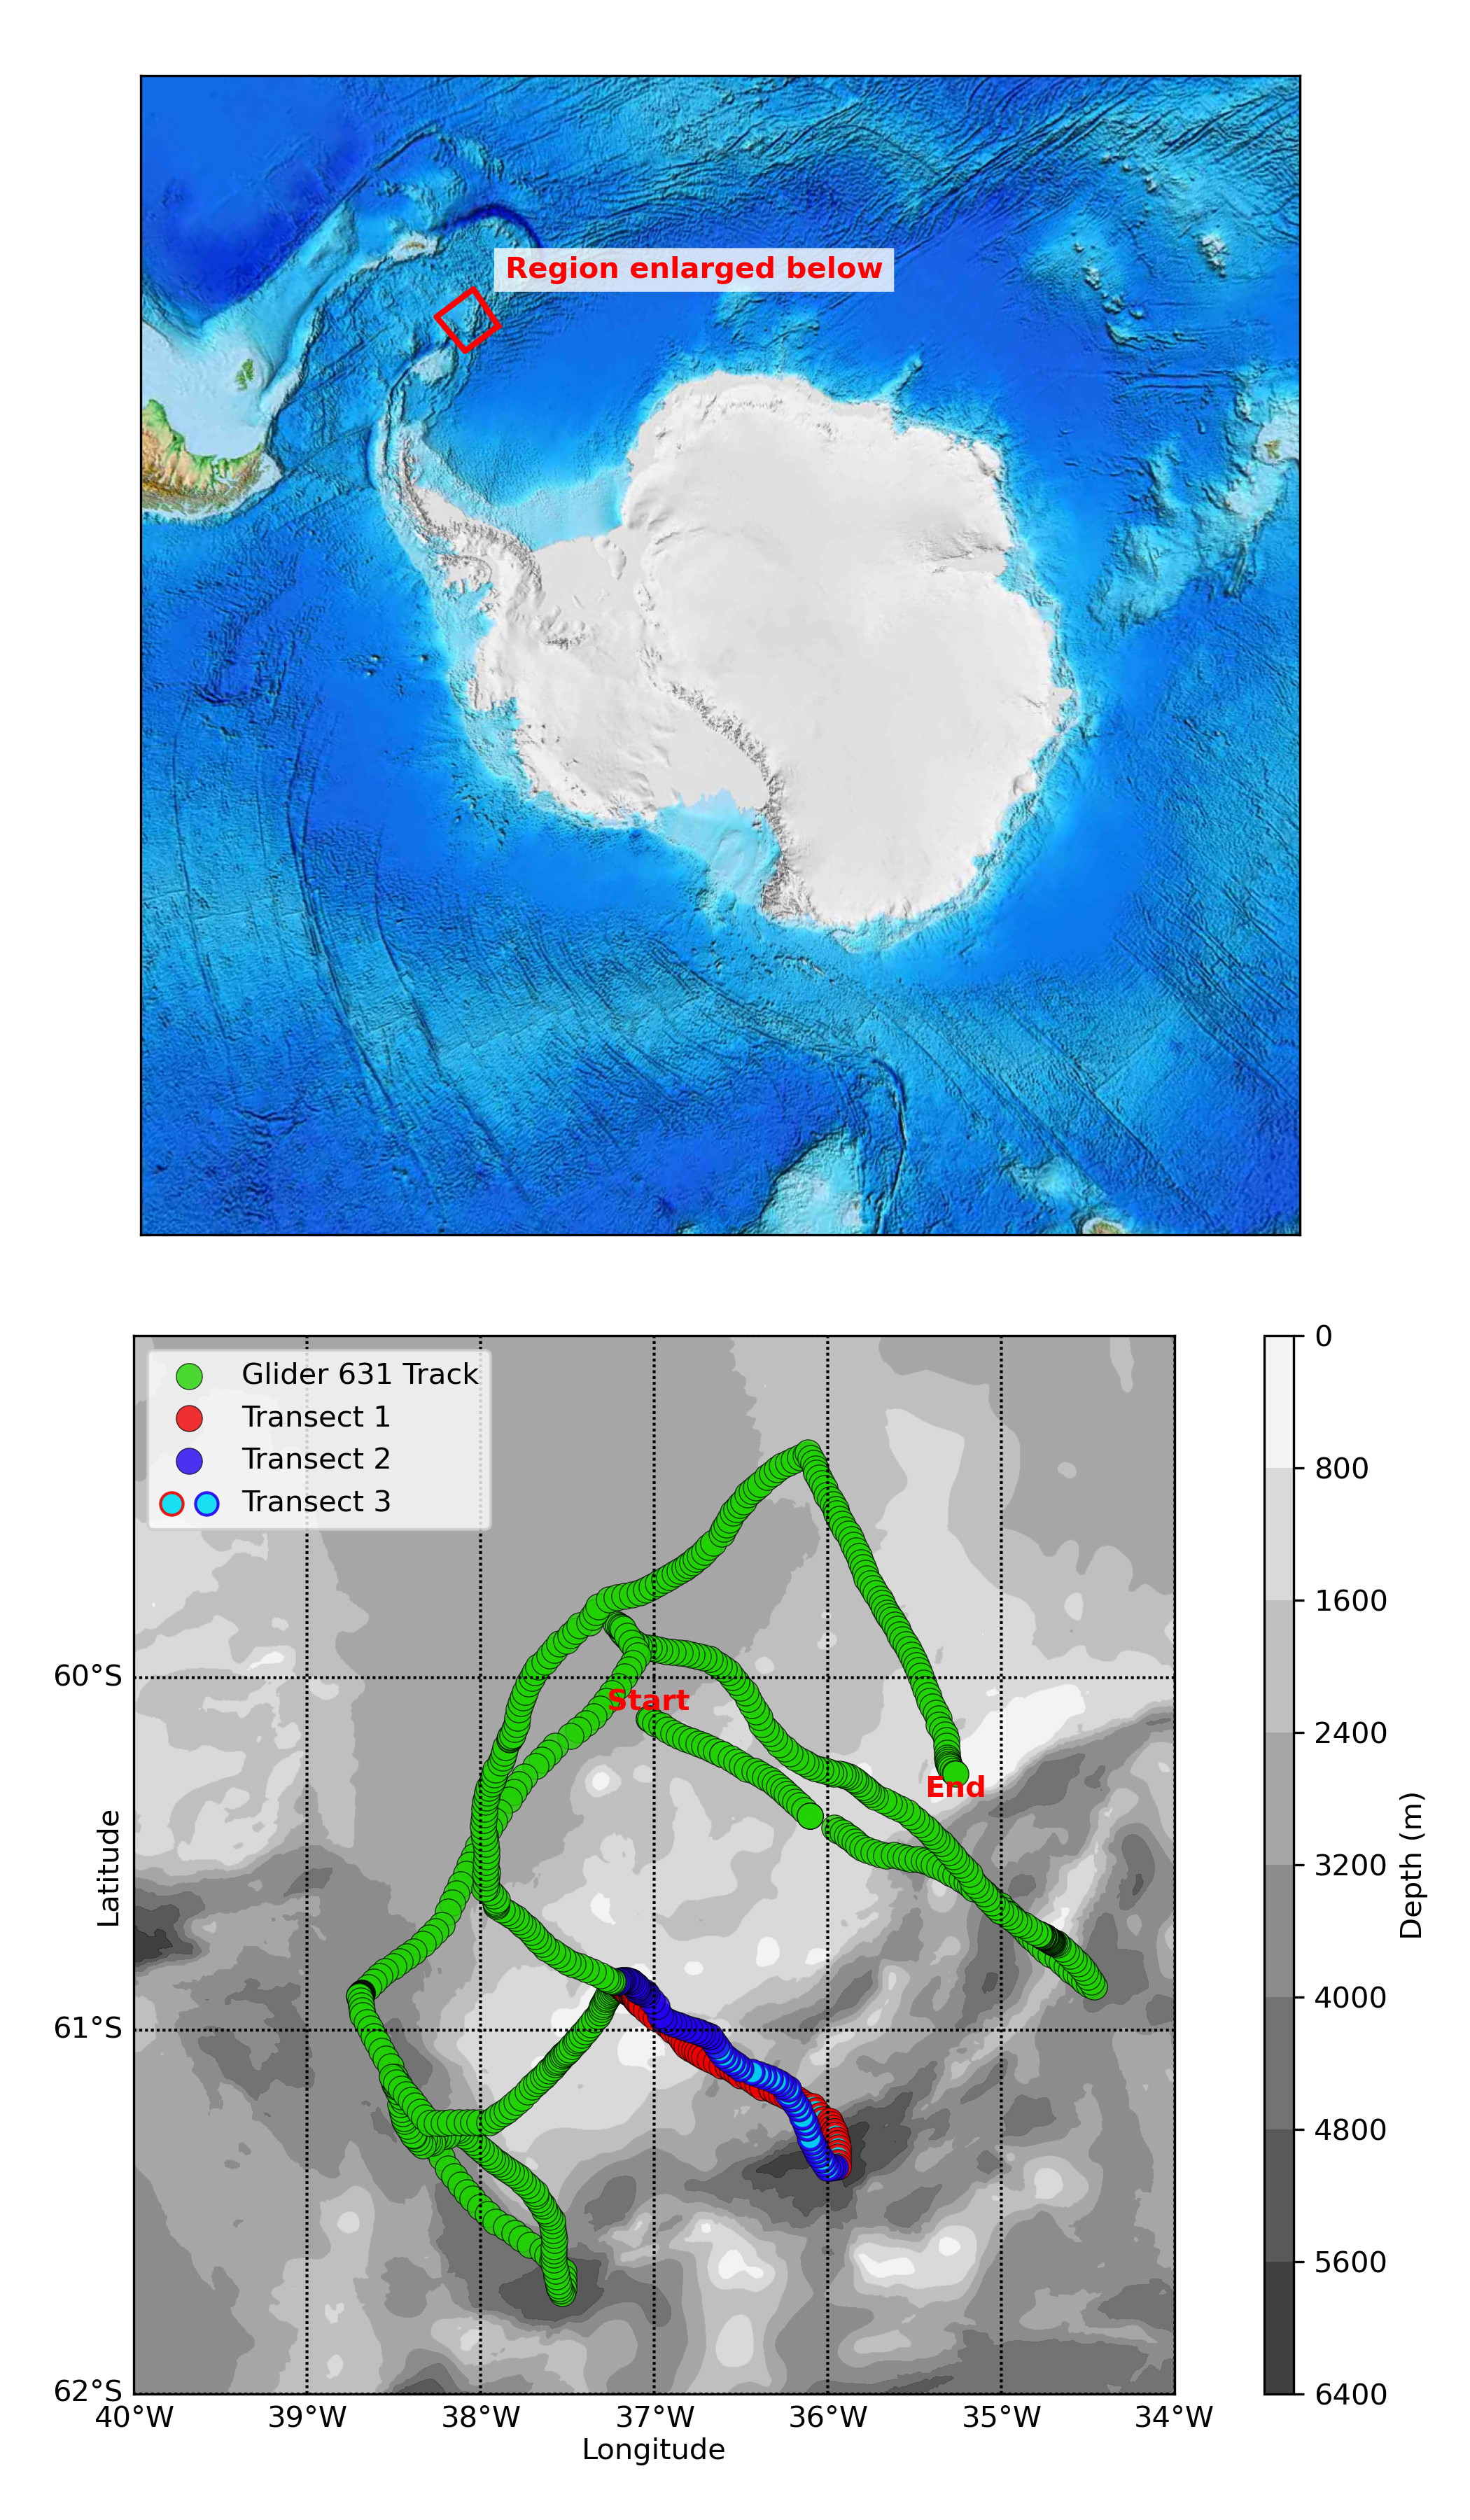
\includegraphics[width=\linewidth]{Louis/figures/figureN.png}
	\caption{\textbf{Location and  Map of glider path.} Red markers denote the data used for Transect 1, a path from the top of the seamount to the deepest contour.
	Dark blue markers denote Transect 2, the return transect. A subset of Transect 1 and 2, Transect 3 is marked with an
	additional cyan dot.}
	\label{fig:N}
\end{figure}

This thesis will primarily examine bio-optical data from the fifth and sixth passes, starting from the location where the fifth
pass began and ending when the sixth pass reached the same location. The fifth pass is labelled Transect 1 and represents the path
from the tip of the seamount out to the deepest area surrounding the mount. Transect 2 is pass six, when the glider returns to the
seamount. Transects 1 and 2 were chosen to provide a full cross-section of the seamount/Taylor column system and are used to
illustrate the effects of bathymetry on productivity. To mitigate the risk of the glider colliding with the sea floor some profiles
within these transects do not extend down to the target depth of 1000 meters. Therefore, Transect 3 was created as a subset of
Transects 1 and 2 where chlorophyll and $b_{bp}$ data was reliably recorded down to 1000 meters and is used as a clear example of the
effects of the data processing steps described in this thesis.


The glider was fitted with a CTD sensor, dissolved oxygen optode, photosynthetically active radiation (PAR) sensor and a WETLabs
EcoPuck containing a coloured dissolved organic matter (CDOM) sensor, an optical backscattering sensor and a fluorometer recording
chlorophyll concentrations \citep{ref1}. The CTD data was compared and corrected against high-quality CTDs. Full details of the
temperature and salinity corrections can be found in \citet{ref2}. The corrected CTD data was used for the calculation of the
mixed layer depth (MLD) as well as conversion of volume backscattering function to the particulate backscattering coefficient. The
PAR data was used for the calculation of photic depth, using the method in \citet{ref42}. Data from the dissolved oxygen optode
and CDOM is not used here.


The majority of the data analysed in this thesis comes from the EcoPuck. The EcoPuck’s fluorometer excites chlorophyll with 470
nm light, which fluoresces to produce light that is detected at 695 nm. This is linearly correlated with chlorophyll concentration
and scaling is used to convert the voltage received from the optical sensor to a concentration in $\mu g l^{-1}$. This takes place
aboard the glider. The backscattering sensor uses a light source offset at 124° from an optical sensor to estimate the total
backscattering of the water. Factors influencing the degree to which a sample of water scatters lights include attributes of the
water itself, suspended particles, dissolved particles and air bubbles. Attenuation due to dissolved materials is negligible within
the red part of the optical spectrum, so light at 700 nm is used \citep{ref3}. Bathymetry data used in this thesis is sourced from
the GEBCO 2024 15 arcsecond dataset \citep{ref7}.


\subsection{3.2. Initial Data Manipulation}
The data was processed within Python, primarily utilising Pandas (written in C) for efficiency. The entire dataset was imported as
a single, continuous dataframe, before being split into a sequence of profiles (with unique profiles for each up and downcast), each
containing their own dataframe with several custom methods for ease of manipulation and to minimise data loaded in memory. Data was
cached after significant preprocessing steps to reduce computation time. General functions were written to be applied to a generic
list of profiles. This means the code could be very easily modified for use with other datasets. Based on profile indicies generated
by the glider, the data could be split into transects representing the different paths and locations the glider traversed, labelled
on Figure \ref{fig:N}. 

\begin{figure}[H] % Two column figure (notice the starred environment)
	\includegraphics[width=\linewidth]{Louis/figures/figureJ.png}
	\caption{\textbf{Flowchart of data processing steps.}}
	\label{fig:J}
\end{figure}

Before the glider data could be used, the following preprocessing steps needed to be taken:
\begin{itemize}
	\item Calculation of accurate salinity and temperature readings.
	\item Mixed layer depth calculation via density anomaly. 
	\item Conversion of volume backscattering function into particulate backscattering coefficient ($b_{bp}$).
	\item Sanitisation of the resulting $b_{bp}$ data using despiking and bubble correcting.
	\item Dark correcting chlorophyll data.
	\item Combining the $b_{bp}$, mixed layer depth and chlorophyll data as part of the chlorophyll quenching correction.
\end{itemize}

Once these steps (in Figure \ref{fig:J} and detailed below) had been completed, the resulting quenching corrected chlorophyll data could be analysed.

\section{4. Methodology and Results}

\subsection{4.1. Calculation of accurate temperature and salinity readings.}
Salinity and temperature were quality-controlled according to the process used in \citet{ref2}, after which the publicly available ‘GSW’
module based on the TEOS-10 equations \citep{ref9} was used in Python to convert the practical salinity into absolute salinity and the
temperature into conservative temperature used for the mixed layer depth calculations.

\subsection{4.2. Conversion of Volume Backscattering Function to \boldmath{$b_{bp}$}.}
The relation between the volume scattering function, $\beta$, and $b_{bp}$ is linear,
with the correlation coefficient, $\chi = 1.077$ \citep{ref5}.
\begin{equation}
	b_{bp} = 2 \pi \chi (\beta - \beta_{sw})
	\label{eq:1}
\end{equation}
$\beta_{sw}$, the background volume scattering coefficient of seawater, was calculated using the method described in \citet{ref6}, using corrected local temperature and
salinity values with the default depolarisation ratio of $\delta$ = 0.039. This required the rewriting of the MATLAB
scripts from \citet{ref6} into Python, allowing the quick conversion of  to $b_{bp}$.

\subsection{4.3. \boldmath{$b_{bp}$} Despiking}

The $b_{bp}$ data contains spikes caused by particles in the water. To remove these, an approach similar to
\citet{ref10} was used, whereby a 7-point running minimum filter followed by a 7-point running maximum was used
to obtain the background readings. Some missing readings within the $b_{bp}$ dataset could not be interpolated,
while large amounts of noise was also present. However, once the data was de-spiked, a simple linear interpolation
over the missing values was applied.

The subsequent de-spiked dataset was then subtracted from the raw data to
obtain the isolated spikes (Figure \ref{fig:D}). Subsequently, a noise threshold was obtained as $8.7 \times 10^{-5} $ m$^{-1}$,
equivalent to the 90th percentile of the entire dataset below 300 meters. Noise from the sensor present in the
spike dataset was removed by setting any values smaller than the noise threshold to zero to allow the spikes to be isolated.
The spike data can be utilised in the future to investigate the fluxes of sinking particulate matter.

\begin{figure}[H] % Two column figure (notice the starred environment)
	\includegraphics[width=\linewidth]{Louis/figures/figureD.png}
	\caption{\textbf{Despiking process.} (a) Raw $b_{bp}$ data in grey with the despiked result in black. (b) isolated spikes in grey with the noise threshold of $8.7 \times 10^{-5} $ m$^{-1}$ as a dotted black line.}
	\label{fig:D}
\end{figure}


\subsection{4.4. Methods for Removing Bubbles}
There is a significant difference in the $b_{bp}$ data between the upcasts
and downcasts. Figure \ref{fig:F} shows that the upcasts are lacking the large $b_{bp}$ values present in the top 100
meters of the profile.


\begin{figure}[H] 
	\includegraphics[width=\linewidth]{Louis/figures/figureF.png}
	\caption{\textbf{Bubble correction for \boldmath{$b_{bp}$}.} (a) $b_{bp}$ plotted against depth for Transect 3 with the shaded region representing the 95\% confidence interval. The average difference between up and downcasts is shown in black. (b) Enlarged view of the difference between up and downcasts with an example of the bubble correction adjustment function overlaid in red.}
	\label{fig:F}
\end{figure}

 
These anomalous datapoints are likely due to air bubbles sticking onto the backscattering sensor
and increasing the amount of light scattered into the detector \citep{ref11}. This discrepancy between the signals
persists throughout the entire downcast, although not to a significant degree beyond 80 meters. To remove these
signals each (de-spiked) downcast is compared to the mean of the six closest de-spiked upcasts. A piecewise function
consisting of multiple linear segments is fitted to the difference between the downcast and its closest upcasts:
\begin{equation}
\label{eq:2}
\begin{split}
	& f(x, y) = y(i) + (y(i+1) - y(i))\times  \frac{x - d(i)}{d(i+1) - d(i)} \\
	& \{ d(i) < x \leq d(i+1) \}  \\
	& d = [0, 10, 20, ..., 150, 160, 999]
\end{split}
\end{equation}

$x$ is the depth while $d$ is an array of depths for the linear segments.
This function is repeated for $i=0$ to $i=15$ such that a correction is created for the entire profile.
The values of $y(i)$ are initially set to the values of $b_{bp}$ at the locations $d(i)$ but are then optimised
(bound to positive values) to create the bubble correction adjustment. This corresponds to a series of sequential
linear fits of the data at ten-meter intervals between zero and 160 meters, as well as a single adjustment between
160-999 meters. The locations of these line segments were chosen to allow for high flexibility in the top 160 meters
(twice the depth at which the discrepancies are commonly seen) while preventing overfitting in the lower 840 meters.
An example of this is shown in Figure \ref{fig:F} (b).

\begin{figure}[H] 
	\includegraphics[width=\linewidth]{Louis/figures/figureG.png}
	\caption{\textbf{Difference between up and downcast \boldmath{$b_{bp}$}.}  Data shown is for Transect 3, both before (red) and after (green) the bubble correction. High frequencies are retained while the large discrepancies in the top 100 meters are significantly reduced.}
	\label{fig:G}
\end{figure}


This function is then subtracted from the raw $b_{bp}$ downcast which is then re-run through the despiking process
to obtain de-spiked, de-bubbled data. The result of this process was a factor of six reduction in mean discrepancy
between the up and downcasts, which increased to over ten within the top 100 meters, as seen in Figure \ref{fig:G}.
Additionally, within Figure \ref{fig:E} (b) visible stripes are seen between consecutive up and downcasts, while
within Figure \ref{fig:E} (c) these stripes are significantly reduced. This difference is most visible within the
top 100 meters where the majority of change is seen between the raw and de-bubbled data.

Some sensitivity analysis was conducted on both the length of the segments in the bubble adjustment and the number
of upcasts used to compare against the downcast. Ten-meter segments provided a balance between efficiency of function
optimization and good results within the top 100 meters - longer segments resulted in worse fits with the upcast data
while shorter segments resulted in overfitting and significantly longer computation times. If fewer than six upcasts
were used for comparison, variability in the difference function was high and optimisation did not always return an
accurate fit. When more upcasts were used in the comparison, changing conditions were no longer accurately represented
in the downcast data. Therefore the smallest number of upcasts that did not create excessive variability, six, was chosen.

\end{multicols}

\begin{figure}[H] 
	\includegraphics[width=\linewidth]{Louis/figures/figureE.png}
	\caption{\boldmath{$b_{bp}$} \textbf{correction stages.}  Transect 3, gridded to two meter intervals. (a) Raw data, before pre-processing. (b) Despiked data. (c) Despiked data following the bubble correction. (d) The noise-filtered spikes extracted from the final despiking process.}
	\label{fig:E}
\end{figure}
\newpage
\begin{multicols}{2}

\subsection{4.5. Chlorophyll Deep Correction}
As the chlorophyll data are determined from a scaled voltage, a correction to the deep values where chlorophyll is expected
to be zero is required. To do this, a deep correction derived from \citet{ref43} is used whereby the 5th percentile of chlorophyll
below 300 meters is subtracted from the entire column (Figure \ref{fig:A}). 
300 meters is well below the photic zone where most chlorophyll is found
and taking the 5th percentile preserves spikes caused by sinking biological matter.
This generates a small number of negative chlorophyll values which are subsequently set to zero.
\begin{figure}[H] 
	\includegraphics[width=\linewidth]{Louis/figures/figureA.png}
	\caption{\textbf{Deep chlorophyll correction.} (main) Chlorophyll concentrations for a profile within Transect 1 before and after the deep correction was applied. (inset) Enlarged view of the same profile, showing the position of the 5th percentile below 300 meters at $0.0511$ mg m$^{-3}$.}
	\label{fig:A}
\end{figure}

\subsection{4.6. Mixed Layer Depth Calculations}
Required for the following chlorophyll quenching correction, the MLD is defined as the point within a profile at which the density
anomaly is greater than $0.03$ kg m$^{-3}$ compared to the density at the surface \citep{ref8}. The surface density was taken as the first
reading when the profile was sorted by depth. Density anomaly was calculated using TEOS-10 calculations applied to the absolute salinity,
conservative temperature and pressure \citep{ref9}. The MLDs were precisely defined as the depth halfway between two data points, where
the first is below the $0.03$ kg m$^{-3}$ threshold while the second is above.
It was decided that $0.03$ kg m$^{-3}$ was a valid choice for the MLDs,
as this value fell within a region where the derivative of density anomaly with depth was high - significant changes to the $0.03$ kg m$^{-3}$
coefficient would be needed to have any meaningful effect on the calculated MLDs. This can be seen in Figure \ref{fig:B} where the line at
$0.03$ kg m$^{-3}$ is in a region where the density anomaly line is steep.

\begin{figure}[H] 
	\includegraphics[width=\linewidth]{Louis/figures/figureB.png}
	\caption{\textbf{Density anomaly.} Density anomaly of the same profile as in Figure \ref{fig:A} . The dashed red line indicates where the density anomaly is $0.03$ kg m$^{-3}$.}
	\label{fig:B}
\end{figure} 

\subsection{4.7. Quenching Correction}
In daytime, observed chlorophyll values are often lower than expected within the top 100 meters. This is caused by the photochemical quenching
used by phytoplankton to protect themselves from excessive light exposure \citep{ref56}. The premise of the quenching correction is to replace
the affected chlorophyll readings with ones derived from the unaffected $b_{bp}$ readings.

To do this, the mean ratio of chlorophyll and bubble corrected, de-spiked $b_{bp}$ within the mixed layer is calculated for the nearest night
upcast. This ratio is then multiplied by the $b_{bp}$ data to create a synthetic chlorophyll reading that is not affected by photochemical
quenching \citep{ref43}. Should this correction provide a value that is lower than the original chlorophyll reading the original reading is
preserved. This method builds upon that used in \citet{ref43}, the key difference being that instead of applying the chlorophyll to backscatter
ratio of the night profile at each depth, the mean ratio of the mixed layer is used. The correction is also applied deeper, across the entire
mixed layer.
\begin{figure}[H] 
	\includegraphics[width=\linewidth]{Louis/figures/figureC.png}
	\caption{\textbf{Quenching correction.} Chlorophyll concentrations for the uncorrected and corrected day profiles (red and green) compared to the night profiles (black) for the entire dataset. Shaded regions indicate the 95\% confidence interval for the respective curve. Correlation coefficients for the day profiles are given with respect to the night profiles.}
	\label{fig:C}
\end{figure}

As can be seen from Figure \ref{fig:C}, this quenching correction improved the correlation between the day and night profiles and the corrected
day profiles are similar in shape to the night ones. The daytime chlorophyll values derived from the correction are reasonable and in line with
expected values for the region. It is expected that the chlorophyll would be more concentrated in the daytime due to the short lifetimes of
algae creating diurnal cycles in chlorophyll concentration \citep{ref57}. Within Figure \ref{fig:H} it is evident that the diurnal decrease in
chlorophyll concentration within the top 30 meters is no longer present after the correction has been applied.
\begin{figure}[H] 
	\includegraphics[width=\linewidth]{Louis/figures/figureH.png}
	\caption{\textbf{Quenching correction result.} Three meter gridded chlorophyll concentrations for Transect 3 before (a) and after (b) the quenching correction is applied. The mixed layer depth is shown as a dotted red line. The daily variation in concentration within the top 30 meters is no longer visible after the correction.}
	\label{fig:H}
\end{figure}
 

\subsection{4.8. High Chlorophyll and Photic Zones}

To quantify the effect of the Taylor column on the productivity of the region, a number of depths were calculated. Firstly, the photic depth
was calculated as where the photosynthetically active radiation (PAR) fell to 1\% of the surface values, interpolating over the night profiles
where insufficient PAR was present to calculate the depth. To complement this, the “High Chlorophyll zone” was calculated - defined as the
location where chlorophyll fell below 3\% of the maximum value within the column, shown in Figure \ref{fig:M}. This quantifies the depth to
which chlorophyll is present. By computing the difference between the photic depth and High Chlorophyll zone we can determine the locations
where additional chlorophyll is present within the water.


\begin{figure}[H] 
	\includegraphics[width=\linewidth]{Louis/figures/figureM.png}
	\caption{\textbf{High Chlorophyll zone and photic depths.} Ten meter gridded chlorophyll concentrations for (a) Transect 1 and (b) Transect 2 with depth of photic zone (black) and depth of ‘High Chlorophyll zone’ (red). The left edges of the plots corresponds to the tip of the seamount and the centre of the Taylor column.}
	\label{fig:M}
\end{figure}


\section{5. Discussion}
\subsection{5.1. Can the effects of bubbles on backscattering data be mitigated?}
The methods described in this paper show that the impact of air bubbles on backscattering data can be effectively mitigated. By using adjustments
based on surrounding unaffected profiles the resultant data maintains local variability. The adjustment also takes into account the degree to
which bubbles affect the data - if there are few bubbles in the water then there will be little difference between up and downcasts and hence
less adjustment. This ensures that it is suitable for long missions where there can be changes in conditions as the seasons change. The ability
to prevent bubbles from affecting data is useful in allowing a greater portion of datasets to be used. This proves invaluable when datasets are
limited and obtaining more data is not easily feasible, such as when the location is remote, i.e. the Southern Ocean.



\end{multicols}

\begin{figure}[H] 
	\includegraphics[width=\linewidth]{Louis/figures/figureK.png}
	\caption{\textbf{Map of productivity metrics.} (left) Map of High Chlorophyll zone depth throughout the glider mission. (right) map of the extent to which the High Chlorophyll zone extends below the Photic Zone depth. GEBCO bathymetry as background.}
	\label{fig:K}
\end{figure}
\begin{multicols}{2}


\subsection{5.2. Is productivity around Discovery Bank affected by the Taylor column?} 
Once the effects of bubbles on $b_{bp}$ data was mitigated and chlorophyll quenching corrections applied, it was possible to map the extent
to which the high chlorophyll zone extends beyond the photic depth, as shown in Figure \ref{fig:K}. 

The extent of the high chlorophyll zone beyond the photic depth is used as a proxy to view the effects of increased diapycnal mixing on the
water column. The presence of chlorophyll beyond the photic depth likely indicates enhanced vertical mixing within the column. For there to be
large quantities of chlorophyll below the photic depth, organic matter must be transported downwards as there is insufficient light for significant
algae growth below the photic depth. The exceptions to this would be regions with greatly enhanced $b_{bp}$ (which would correlate with sinking
dead organic matter) or regions where a deep chlorophyll maximum (DCM) is present, which would require phytoplankton adapted to low light
conditions, common in low-latitude oceans \citep{ref58}. As neither of these are present in the data seen around the seamount,
it is reasonable to conclude that the presence of chlorophyll below the photic zone is indicative of enhanced diapycnal mixing.

Figure \ref{fig:K} shows the effect of the seamount (located at 37°W 61°S) on the surrounding region. There are regions where the high chlorophyll
zones are significantly deeper than the photic depth around the 3,200 meter contours surrounding the seamount peak. This aligns with the expected boundaries
of a Taylor column predicted by \citet{ref2} as occurring at about the 3,000 meter contours. These high-productivity regions are therefore likely to have increased
diapycnal mixing around the boundaries of the Taylor column, increasing the flux of nutrients towards the surface and mixing the existing chlorophyll deeper into
the ocean. This is supported by the lower $b_{bp}$ in the surface of these regions, showing that there is more mixing between the particle-dense surface region
and the deeper regions with more sparsely distributed particulate matter.


These regions are then contrasted by lower productivity within the centre of the Taylor column. The regions between the 1,600 and 2,400 meter
contours do not show enhanced chlorophyll concentrations within the 100 to 200 meter depth region, see Figure \ref{fig:I} (a). This implies the existence
of a region with increased water residence times, to the extent that productivity may be limited by nutrient availability. To confirm this,
comparisons need to be made to data acquired in the open ocean in a location within minimal underwater features.

It is therefore likely that both processes (increased diapycnal mixing and increased residence times) are present within the Taylor column.
In the central region, the lack of nutrients due to the long water residence time is the dominant factor. Conversely, on the boundaries of the
column, the residence times are likely shorter, and the diapycnal mixing provides nutrients from the deep while also mixing chlorophyll into the
deeper water, which results in deeper regions of high chlorophyll concentrations. 

\end{multicols}
\begin{figure}[H] 
	\includegraphics[width=\linewidth]{Louis/figures/figureI.png}
	\caption{\textbf{Effects of bathymetry on chlorophyll and} \boldmath{$b_{bp}$.}  (a, b) Three meter gridded chlorophyll concentration for Transect 1 and 2 respectively. (c, d) Three meter gridded $b_{bp}$ data for Transect 1 and 2 respectively. (e, f) Depth data interpolated from GEBCO bathymetry. The left edges of the plots corresponds to the tip of the seamount and the centre of the Taylor column.}
	\label{fig:I}
\end{figure}
\begin{multicols}{2}


\subsection{5.3. Future Options}
During the cruise, there were unfortunately no water samples taken against which to calibrate biogeochemical data. Bottle samples, either
returned to a laboratory or analysed onboard the ship, would have provided a reference reading that we could confirm is unaffected by bubbles.
By taking a sample in the same location as a bubble-affected downcast, either at the start or end of the mission, the accuracy of the bubble
correction could be quantified. Ascertaining the quality of this bubble correction would be useful before applying it to other datasets. Future
studies could confirm this by applying it to datasets where reference samples were taken and analysed in a laboratory.

To help quantify the effects of the Taylor column on water residence times and hence on productivity, chlorophyll within the column could be
compared to chlorophyll in the open ocean. If chlorophyll concentrations within the column are significantly lower than in the open ocean it
would indicate that the long residence times are affecting the availability of nutrients within the bounds of the column. This could potentially
be conducted using satellite data but preferably would be done using gliders so that the vertical profiles of chlorophyll in nearby open oceans
can be compared. Future glider missions could also further elucidate the exact mixing processes occurring in the boundaries of the column. It
would be recommended for a glider to revisit the same transects more than once within a deployment to ensure that transient temporal anomalies
are not affecting the data. If a longer mission using several sequential glider deployments were to be conducted, the interactions between the
different seasons and the Taylor column could be investigated, although sea conditions in the austral winter could cause difficulties in reliably
recovering and deploying the gliders. Repeat transects would also allow the comparison of data in the same location over time and enable one to
establish a value for the sinking speed of particulate matter and then ascertain a rate at which carbon is sinking in the vicinity of the Taylor
column.

\subsection{5.4. Importance of solving this problem}
Accurate measurements of chlorophyll and particulate matter within the ocean are crucial for understanding the rates at which organic matter is
sinking. Knowledge of this rate can in turn help determine the efficiency at which the ocean stores carbon and is crucial in guiding climate policy
decisions.

Within the particulate backscattering data, bubbles would artificially increase the concentration of particulate matter within the water.
When quenching corrections are applied, these incorrectly high readings of $b_{bp}$ would increase the calculated chlorophyll concentrations,
thereby overestimating productivity metrics within the photic zone. This could potentially lead to inaccurately low values for the sinking flux
of carbon, downplaying the significance of the ocean in global policy decisions regarding climate change. As such the understanding of the
effects of bubbles on $b_{bp}$ and chlorophyll data is key in ensuring reliable estimates of carbon sequestration are calculated.

\section{6. Conclusion}

The ocean plays a critical role in the global carbon cycle, and oceanographic data drawn from buoyancy gliders can be utilised in informing
policy decisions. Gliders present a unique solution to improving the temporal and spatial ranges over which data can be collected, providing
novel insights into the transformations and mixing processes occurring within the ocean. This thesis has shown that errors in particulate
backscattering coefficients caused by air bubbles on the bio-optical sensors can be mitigated, reducing the discrepancies between up and downcasts 
by a factor of six, allowing a greater portion of acquired glider data to be used in analysis. Having mitigated against these errors, the analysis
is then able to reveal that the Taylor column above Discovery Bank does affect local productivity. There is strong evidence that there is increased
diapycnal mixing within the boundaries of the Taylor column, creating a ring of enhanced productivity around the seamount. Meanwhile, there is also
some limited evidence that the centre of the Taylor column has increased water residence times, indicated by the shallower region of high 
chlorophyll. To further investigate this, comparisons to the open ocean, perhaps using satellite-derived concentrations, would have to be conducted.
Overall, Taylor columns clearly affect the local productivity around seamounts and the degree to which this affects the rate of carbon sinking
into the deep ocean should be a priority for future investigations. Thus this analysis advances methodologies for glider data processing and
provides insights into the impacts of the hydrodynamics surrounding seamounts on biological productivity, with implications for understanding
ocean carbon sequestration and informing climate policy.


\end{multicols}
\vfill{}




\begin{center}
	\rule{\linewidth}{0.4pt}
\end{center}
\section*{Acknowledgements}
	
The writing of this thesis would not have been possible without the support of my supervisors, Prof. Kate Hendry and 
Dr Alex Brearley, who provided invaluable guidance and support throughout the project.
I would also like to thank those who provided advice and feedback during the data analysis and write up process, namely
Dr Natasha Lucas and Dr Nathan Briggs.\\

$c_{\text{new}} = b_{\text{bp}} \times \overline{\frac{c_{\text{night}}}{b_{\text{bp, night}}}}$

\section*{Code and Data Availability}
\urlstyle{same}
The code used in this analysis is available at: \url{https://github.com/louis-de-neve/gliders25/tree/main/Louis}\\
The data used in this analysis is not currently publicly available.\\



%----------------------------------------------------------------------------------------
%	 REFERENCES
%----------------------------------------------------------------------------------------
\renewbibmacro{in:}{}
\clearpage

\twocolumn

	
\printbibliography % Output the bibliography
	

%----------------------------------------------------------------------------------------

\end{document}

